\chapter{\label{ch:x-misc}Miscellaneous notes}

\minitoc

\section{ORION experiment} 
The following derivation determines the polarisation of the ORION laser pulses in the experiment and the boostes frame quantities for the PIC simulations.

I will have a whole subsection devoted to the different frames of reference of relevance and then a second one about normalised units. What follows now is the derivation of the boosted frame in which the laser is incident normally relative to the lab frame where the laser is incident obliquely.

I will try to use a consistent convention for coordinate system as much as possible.

\subsection{Frames of reference}
I should go over this and use third year relativity notes to formalised and make more consistent.

While some of this section may seem trivial, it is frequently miscalculated in the literature, it therefore seems of great importance to provide a full derivation.

Consider a photon incident on a plasma block at angle $\theta$ as in figure \ref{fig:miscreferenceframesboosted1d}.
% TODO: \usepackage{graphicx} required
\begin{figure}
	\centering
	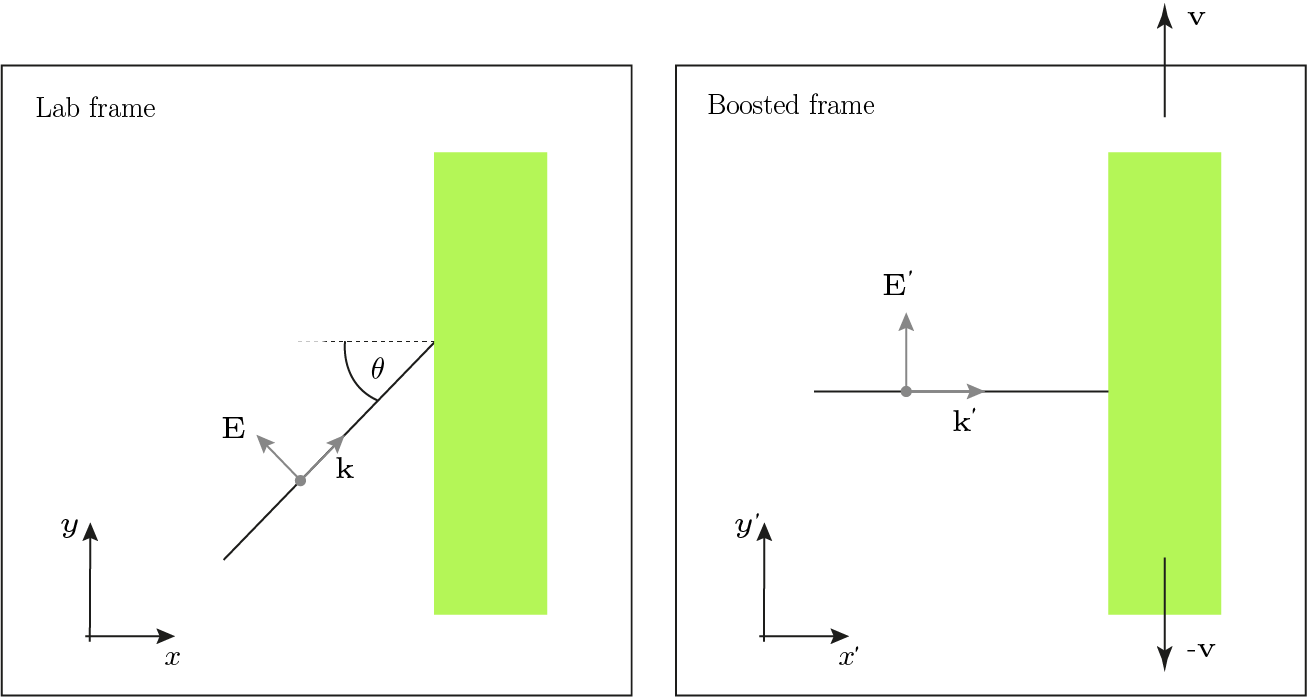
\includegraphics[width=1\linewidth]{figures/misc/misc_reference_frames_boosted_1D}
	\caption{}
	\label{fig:miscreferenceframesboosted1d}
\end{figure}
A boost is applied with velocity $\mathbf{v}$ to a frame such that the photon is normally incident on the now streaming plasma at velocity $-\mathbf{v}$. The velocity transformation for the photon's velocity, $\mathbf{u}$, parallel to the boost is
\begin{equation}
	\mathbf{u}'_\parallel = \frac{\mathbf{u}_\parallel - \mathbf{v}}{1-\mathbf{u}\cdot\mathbf{v}/c^2}.
\end{equation}
Setting  $\mathbf{u}'_\parallel = 0$, it is clear that
\begin{equation}
	\mathbf{v} = \mathbf{u}_\parallel = c\sin\theta \hat{\mathbf{y}}
\end{equation}
in this geometry and 
\begin{equation}
	\gamma_\mathbf{v} = \frac{1}{\sqrt{1-\mathbf{v}^2/c^2}}=\sec\theta.
\end{equation}
Noting that since Snell's law is frame invariant, the photon remains normal as it propagates into the skin depth of the plasma, a frame in which the interaction reduces to a 1D problem has been successfully found for all $\theta < \pi/2$. Those familiar with the topic may wonder how this is possible considering the `ripples' that are observed on the plasma surface for oblique incidence. The explanation for this is of course the relativity of simultaneity. It remains to determine how do all the relevant quantities transform as such a boost is applied. Starting with an easy one: the photon's wave four-vector is 
\begin{equation}
	\mathbf{K}^\mathrm{\mu} = \left(\frac{\omega}{c},\mathbf{k}\right)
\end{equation}
and thus the freqency transforms as
\begin{equation}
	\frac{\omega}{c} = \gamma_\mathbf{v}\left(\frac{\omega'}{c}-\frac{\mathbf{v}}{c}\cdot\mathbf{k'}\right).
\end{equation}
Since $\mathbf{v}\cdot\mathbf{k'} = 0$, 
\begin{equation}\label{eq:boost_omega}
	\omega' = \omega\cos\theta .
\end{equation}
As 
\begin{equation}
	n'_\mathrm{c} = \frac{m_\mathrm{e}(\omega')^2}{4\pi e^2},
\end{equation}
\begin{equation}\label{eq:boost_nc}
	n'_\mathrm{c} =n_\mathrm{c} \cos^2\theta ,
\end{equation}
while the plasma block will be Lorentz contracted along $\hat{\mathbf{y}}$, hence the number density of electrons will increase as,
\begin{equation}
	n'_\mathrm{e} = \frac{n'_\mathrm{e}}{\cos\theta},
\end{equation}
leading to the perhaps unexpected
\begin{equation}
	\bar{n}'_\mathrm{e} = \frac{\bar{n}_\mathrm{e}}{\cos^3\theta}.
\end{equation}


Consider now the more general case (I should jsut simply replace my diagram with a 3D one that incorporates this initially) where the photon's electric field is rotated out of the $x$-$y$ plane, \textit{i.e.}
\begin{equation}
	\mathbf{E} = E_0(-\cos\phi\sin\theta,\cos\phi\cos\theta,\sin\phi)
\end{equation}
and correspondingly
\begin{equation}
	\mathbf{B} = \frac{\hat{\mathbf{k}} \times \mathbf{E}}{c}= \frac{E_0}{c}(\sin\phi\sin\theta,-\sin\phi\cos\theta,\cos\phi).
\end{equation}
The Lorentz transformations for electro-magnetic fields are
\begin{equation}
	\mathbf{E}'_\parallel = \mathbf{E}_\parallel,
\end{equation}
\begin{equation}
	\mathbf{B}'_\parallel = \mathbf{B}_\parallel,
\end{equation}
\begin{equation}
	\mathbf{E}'_\perp = \gamma_\mathbf{v}(\mathbf{E}_\perp + \mathbf{v} \times \mathbf{B}),
\end{equation}
\begin{equation}
	\mathbf{B}'_\perp = \gamma_\mathbf{v}(\mathbf{B}_\perp - \mathbf{v} \times \mathbf{E}/c^2).
\end{equation}
Using the above expressions for $\mathbf{E}_\perp$ and $\mathbf{E}_\parallel$ and transforming to the boosted frame,
\begin{equation}
	\mathbf{E}' = E_0\cos\theta (0,\cos\phi,\sin\phi).
\end{equation}
As anticipated for normal incidence there is no component of the E-field normal to the surface. Conveniently, the polarisation of the incident photon is unchanged despite having components both parallel and perpendicular to the transformation and 
\begin{equation}
	|\mathbf{E}'| = |\mathbf{E}|\cos\theta.
\end{equation}
The picture can now be completed. Since
\begin{equation}
	a_0' = \frac{e|\mathbf{E}'|}{m_\mathrm{e}e\omega'}
\end{equation}
it follows that
\begin{equation}
	a_0' = a_0,
\end{equation}
\begin{equation}
	S' = \frac{S}{\cos^3\theta}.
\end{equation}

Also discuss the fabulous result that generally one can simply extract the results in the Smilei units and multiply by the relevant factors of the frame of interest and thus not worry too much about frame transformations.




Once I have finished this section I must redo boosted section since I have made a mistake there and rethink a bit about optimum theta.

I must also at some point just state that a hat indicates a normalised vector.

